\documentclass[1p]{elsarticle_modified}
%\bibliographystyle{elsarticle-num}

%\usepackage[colorlinks]{hyperref}
%\usepackage{abbrmath_seonhwa} %\Abb, \Ascr, \Acal ,\Abf, \Afrak
\usepackage{amsfonts}
\usepackage{amssymb}
\usepackage{amsmath}
\usepackage{amsthm}
\usepackage{scalefnt}
\usepackage{amsbsy}
\usepackage{kotex}
\usepackage{caption}
\usepackage{subfig}
\usepackage{color}
\usepackage{graphicx}
\usepackage{xcolor} %% white, black, red, green, blue, cyan, magenta, yellow
\usepackage{float}
\usepackage{setspace}
\usepackage{hyperref}

\usepackage{tikz}
\usetikzlibrary{arrows}

\usepackage{multirow}
\usepackage{array} % fixed length table
\usepackage{hhline}

%%%%%%%%%%%%%%%%%%%%%
\makeatletter
\renewcommand*\env@matrix[1][\arraystretch]{%
	\edef\arraystretch{#1}%
	\hskip -\arraycolsep
	\let\@ifnextchar\new@ifnextchar
	\array{*\c@MaxMatrixCols c}}
\makeatother %https://tex.stackexchange.com/questions/14071/how-can-i-increase-the-line-spacing-in-a-matrix
%%%%%%%%%%%%%%%

\usepackage[normalem]{ulem}

\newcommand{\msout}[1]{\ifmmode\text{\sout{\ensuremath{#1}}}\else\sout{#1}\fi}
%SOURCE: \msout is \stkout macro in https://tex.stackexchange.com/questions/20609/strikeout-in-math-mode

\newcommand{\cancel}[1]{
	\ifmmode
	{\color{red}\msout{#1}}
	\else
	{\color{red}\sout{#1}}
	\fi
}

\newcommand{\add}[1]{
	{\color{blue}\uwave{#1}}
}

\newcommand{\replace}[2]{
	\ifmmode
	{\color{red}\msout{#1}}{\color{blue}\uwave{#2}}
	\else
	{\color{red}\sout{#1}}{\color{blue}\uwave{#2}}
	\fi
}

\newcommand{\Sol}{\mathcal{S}} %segment
\newcommand{\D}{D} %diagram
\newcommand{\A}{\mathcal{A}} %arc


%%%%%%%%%%%%%%%%%%%%%%%%%%%%%5 test

\def\sl{\operatorname{\textup{SL}}(2,\Cbb)}
\def\psl{\operatorname{\textup{PSL}}(2,\Cbb)}
\def\quan{\mkern 1mu \triangleright \mkern 1mu}

\theoremstyle{definition}
\newtheorem{thm}{Theorem}[section]
\newtheorem{prop}[thm]{Proposition}
\newtheorem{lem}[thm]{Lemma}
\newtheorem{ques}[thm]{Question}
\newtheorem{cor}[thm]{Corollary}
\newtheorem{defn}[thm]{Definition}
\newtheorem{exam}[thm]{Example}
\newtheorem{rmk}[thm]{Remark}
\newtheorem{alg}[thm]{Algorithm}

\newcommand{\I}{\sqrt{-1}}
\begin{document}

%\begin{frontmatter}
%
%\title{Boundary parabolic representations of knots up to 8 crossings}
%
%%% Group authors per affiliation:
%\author{Yunhi Cho} 
%\address{Department of Mathematics, University of Seoul, Seoul, Korea}
%\ead{yhcho@uos.ac.kr}
%
%
%\author{Seonhwa Kim} %\fnref{s_kim}}
%\address{Center for Geometry and Physics, Institute for Basic Science, Pohang, 37673, Korea}
%\ead{ryeona17@ibs.re.kr}
%
%\author{Hyuk Kim}
%\address{Department of Mathematical Sciences, Seoul National University, Seoul 08826, Korea}
%\ead{hyukkim@snu.ac.kr}
%
%\author{Seokbeom Yoon}
%\address{Department of Mathematical Sciences, Seoul National University, Seoul, 08826,  Korea}
%\ead{sbyoon15@snu.ac.kr}
%
%\begin{abstract}
%We find all boundary parabolic representation of knots up to 8 crossings.
%
%\end{abstract}
%\begin{keyword}
%    \MSC[2010] 57M25 
%\end{keyword}
%
%\end{frontmatter}

%\linenumbers
%\tableofcontents
%
\newcommand\colored[1]{\textcolor{white}{\rule[-0.35ex]{0.8em}{1.4ex}}\kern-0.8em\color{red} #1}%
%\newcommand\colored[1]{\textcolor{white}{ #1}\kern-2.17ex	\textcolor{white}{ #1}\kern-1.81ex	\textcolor{white}{ #1}\kern-2.15ex\color{red}#1	}

{\Large $\underline{12n_{0410}~(K12n_{0410})}$}

\setlength{\tabcolsep}{10pt}
\renewcommand{\arraystretch}{1.6}
\vspace{1cm}\begin{tabular}{m{100pt}>{\centering\arraybackslash}m{274pt}}
\multirow{5}{120pt}{
	\centering
	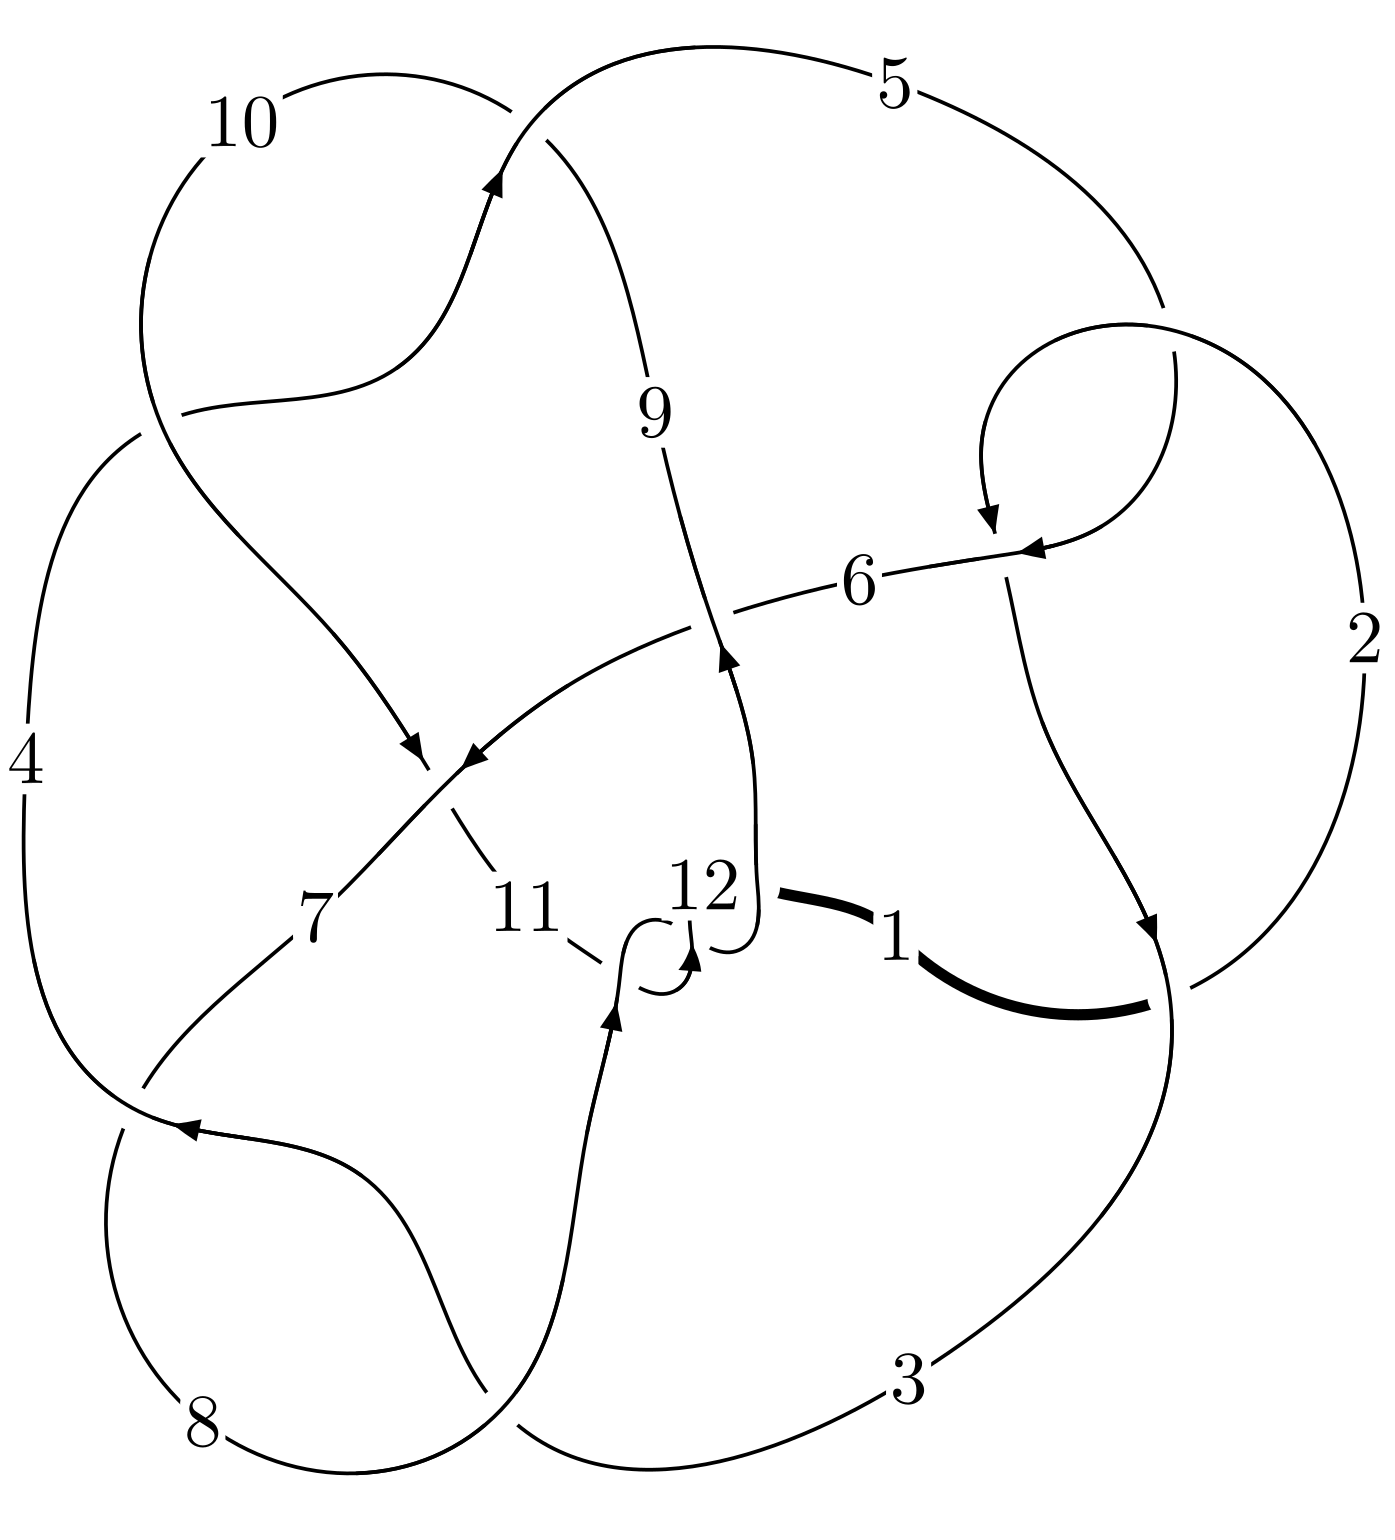
\includegraphics[width=112pt]{../../../GIT/diagram.site/Diagrams/png/2499_12n_0410.png}\\
\ \ \ A knot diagram\footnotemark}&
\allowdisplaybreaks
\textbf{Linearized knot diagam} \\
\cline{2-2}
 &
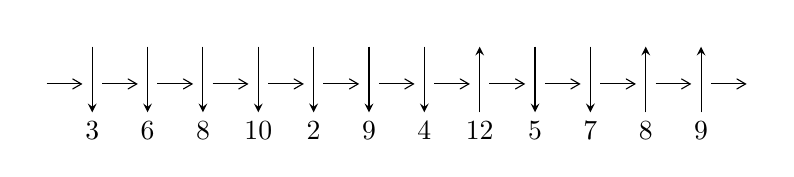
\begin{tikzpicture}[x=20pt, y=17pt]
	% nodes
	\node (C0) at (0, 0) {};
	\node (C1) at (1, 0) {};
	\node (C1U) at (1, +1) {};
	\node (C1D) at (1, -1) {3};

	\node (C2) at (2, 0) {};
	\node (C2U) at (2, +1) {};
	\node (C2D) at (2, -1) {6};

	\node (C3) at (3, 0) {};
	\node (C3U) at (3, +1) {};
	\node (C3D) at (3, -1) {8};

	\node (C4) at (4, 0) {};
	\node (C4U) at (4, +1) {};
	\node (C4D) at (4, -1) {10};

	\node (C5) at (5, 0) {};
	\node (C5U) at (5, +1) {};
	\node (C5D) at (5, -1) {2};

	\node (C6) at (6, 0) {};
	\node (C6U) at (6, +1) {};
	\node (C6D) at (6, -1) {9};

	\node (C7) at (7, 0) {};
	\node (C7U) at (7, +1) {};
	\node (C7D) at (7, -1) {4};

	\node (C8) at (8, 0) {};
	\node (C8U) at (8, +1) {};
	\node (C8D) at (8, -1) {12};

	\node (C9) at (9, 0) {};
	\node (C9U) at (9, +1) {};
	\node (C9D) at (9, -1) {5};

	\node (C10) at (10, 0) {};
	\node (C10U) at (10, +1) {};
	\node (C10D) at (10, -1) {7};

	\node (C11) at (11, 0) {};
	\node (C11U) at (11, +1) {};
	\node (C11D) at (11, -1) {8};

	\node (C12) at (12, 0) {};
	\node (C12U) at (12, +1) {};
	\node (C12D) at (12, -1) {9};
	\node (C13) at (13, 0) {};

	% arrows
	\draw[->,>={angle 60}]
	(C0) edge (C1) (C1) edge (C2) (C2) edge (C3) (C3) edge (C4) (C4) edge (C5) (C5) edge (C6) (C6) edge (C7) (C7) edge (C8) (C8) edge (C9) (C9) edge (C10) (C10) edge (C11) (C11) edge (C12) (C12) edge (C13) ;	\draw[->,>=stealth]
	(C1U) edge (C1D) (C2U) edge (C2D) (C3U) edge (C3D) (C4U) edge (C4D) (C5U) edge (C5D) (C6U) edge (C6D) (C7U) edge (C7D) (C8D) edge (C8U) (C9U) edge (C9D) (C10U) edge (C10D) (C11D) edge (C11U) (C12D) edge (C12U) ;
	\end{tikzpicture} \\
\hhline{~~} \\& 
\textbf{Solving Sequence} \\ \cline{2-2} 
 &
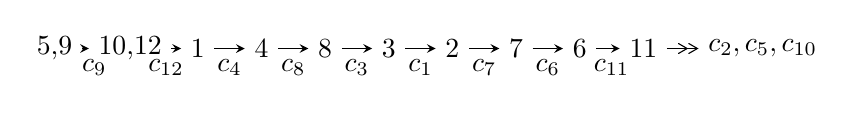
\begin{tikzpicture}[x=23pt, y=7pt]
	% node
	\node (A0) at (-1/8, 0) {5,9};
	\node (A1) at (17/16, 0) {10,12};
	\node (A2) at (17/8, 0) {1};
	\node (A3) at (25/8, 0) {4};
	\node (A4) at (33/8, 0) {8};
	\node (A5) at (41/8, 0) {3};
	\node (A6) at (49/8, 0) {2};
	\node (A7) at (57/8, 0) {7};
	\node (A8) at (65/8, 0) {6};
	\node (A9) at (73/8, 0) {11};
	\node (C1) at (1/2, -1) {$c_{9}$};
	\node (C2) at (13/8, -1) {$c_{12}$};
	\node (C3) at (21/8, -1) {$c_{4}$};
	\node (C4) at (29/8, -1) {$c_{8}$};
	\node (C5) at (37/8, -1) {$c_{3}$};
	\node (C6) at (45/8, -1) {$c_{1}$};
	\node (C7) at (53/8, -1) {$c_{7}$};
	\node (C8) at (61/8, -1) {$c_{6}$};
	\node (C9) at (69/8, -1) {$c_{11}$};
	\node (A10) at (11, 0) {$c_{2},c_{5},c_{10}$};

	% edge
	\draw[->,>=stealth]	
	(A0) edge (A1) (A1) edge (A2) (A2) edge (A3) (A3) edge (A4) (A4) edge (A5) (A5) edge (A6) (A6) edge (A7) (A7) edge (A8) (A8) edge (A9) ;
	\draw[->>,>={angle 60}]	
	(A9) edge (A10);
\end{tikzpicture} \\ 

\end{tabular} \\

\footnotetext{
The image of knot diagram is generated by the software ``\textbf{Draw programme}" developed by Andrew Bartholomew(\url{http://www.layer8.co.uk/maths/draw/index.htm\#Running-draw}), where we modified some parts for our purpose(\url{https://github.com/CATsTAILs/LinksPainter}).
}\phantom \\ \newline 
\centering \textbf{Ideals for irreducible components\footnotemark of $X_{\text{par}}$} 
 
\begin{align*}
I^u_{1}&=\langle 
-3.43647\times10^{106} u^{70}+9.27917\times10^{106} u^{69}+\cdots+4.05492\times10^{107} b-2.66090\times10^{107},\\
\phantom{I^u_{1}}&\phantom{= \langle  }-2.33553\times10^{108} u^{70}-2.92909\times10^{108} u^{69}+\cdots+4.05492\times10^{107} a+1.64345\times10^{109},\\
\phantom{I^u_{1}}&\phantom{= \langle  }u^{71}+u^{70}+\cdots-18 u+1\rangle \\
I^u_{2}&=\langle 
u^2+b+1,\;u^{15}+u^{14}+\cdots+a-4,\\
\phantom{I^u_{2}}&\phantom{= \langle  }u^{16}+10 u^{14}+40 u^{12}+u^{11}+82 u^{10}+7 u^9+92 u^8+18 u^7+58 u^6+21 u^5+25 u^4+11 u^3+10 u^2+2 u+1\rangle \\
\\
\end{align*}
\raggedright * 2 irreducible components of $\dim_{\mathbb{C}}=0$, with total 87 representations.\\
\footnotetext{All coefficients of polynomials are rational numbers. But the coefficients are sometimes approximated in decimal forms when there is not enough margin.}
\newpage
\renewcommand{\arraystretch}{1}
\centering \section*{I. $I^u_{1}= \langle -3.44\times10^{106} u^{70}+9.28\times10^{106} u^{69}+\cdots+4.05\times10^{107} b-2.66\times10^{107},\;-2.34\times10^{108} u^{70}-2.93\times10^{108} u^{69}+\cdots+4.05\times10^{107} a+1.64\times10^{109},\;u^{71}+u^{70}+\cdots-18 u+1 \rangle$}
\flushleft \textbf{(i) Arc colorings}\\
\begin{tabular}{m{7pt} m{180pt} m{7pt} m{180pt} }
\flushright $a_{5}=$&$\begin{pmatrix}0\\u\end{pmatrix}$ \\
\flushright $a_{9}=$&$\begin{pmatrix}1\\0\end{pmatrix}$ \\
\flushright $a_{10}=$&$\begin{pmatrix}1\\u^2\end{pmatrix}$ \\
\flushright $a_{12}=$&$\begin{pmatrix}5.75975 u^{70}+7.22354 u^{69}+\cdots+413.326 u-40.5299\\0.0847481 u^{70}-0.228837 u^{69}+\cdots-1.63551 u+0.656214\end{pmatrix}$ \\
\flushright $a_{1}=$&$\begin{pmatrix}5.84450 u^{70}+6.99470 u^{69}+\cdots+411.690 u-39.8736\\0.0847481 u^{70}-0.228837 u^{69}+\cdots-1.63551 u+0.656214\end{pmatrix}$ \\
\flushright $a_{4}=$&$\begin{pmatrix}u\\u^3+u\end{pmatrix}$ \\
\flushright $a_{8}=$&$\begin{pmatrix}3.49699 u^{70}+4.19855 u^{69}+\cdots+350.333 u-33.4246\\0.239548 u^{70}+0.356147 u^{69}+\cdots+3.79911 u+0.0294177\end{pmatrix}$ \\
\flushright $a_{3}=$&$\begin{pmatrix}0.732278 u^{70}+1.28940 u^{69}+\cdots+57.6526 u-22.5177\\-0.0601700 u^{70}-0.435875 u^{69}+\cdots+18.4320 u-2.09649\end{pmatrix}$ \\
\flushright $a_{2}=$&$\begin{pmatrix}-3.03287 u^{70}-3.14673 u^{69}+\cdots-288.328 u+33.4675\\0.443733 u^{70}+0.847315 u^{69}+\cdots-10.9879 u+0.729411\end{pmatrix}$ \\
\flushright $a_{7}=$&$\begin{pmatrix}3.33586 u^{70}+3.74761 u^{69}+\cdots+351.145 u-33.2572\\0.284126 u^{70}+0.525249 u^{69}+\cdots-0.443567 u+0.486594\end{pmatrix}$ \\
\flushright $a_{6}=$&$\begin{pmatrix}3.61999 u^{70}+4.27286 u^{69}+\cdots+350.702 u-32.7706\\0.284126 u^{70}+0.525249 u^{69}+\cdots-0.443567 u+0.486594\end{pmatrix}$ \\
\flushright $a_{11}=$&$\begin{pmatrix}3.08919 u^{70}+3.79307 u^{69}+\cdots+183.569 u-16.3818\\-0.264976 u^{70}-0.884934 u^{69}+\cdots-4.44816 u+0.538795\end{pmatrix}$\\&\end{tabular}
\flushleft \textbf{(ii) Obstruction class $= -1$}\\~\\
\flushleft \textbf{(iii) Cusp Shapes $= -0.714658 u^{70}+0.411160 u^{69}+\cdots-172.611 u+3.21683$}\\~\\
\newpage\renewcommand{\arraystretch}{1}
\flushleft \textbf{(iv) u-Polynomials at the component}\newline \\
\begin{tabular}{m{50pt}|m{274pt}}
Crossings & \hspace{64pt}u-Polynomials at each crossing \\
\hline $$\begin{aligned}c_{1}\end{aligned}$$&$\begin{aligned}
&u^{71}+37 u^{70}+\cdots+39 u+1
\end{aligned}$\\
\hline $$\begin{aligned}c_{2},c_{5}\end{aligned}$$&$\begin{aligned}
&u^{71}+u^{70}+\cdots-5 u+1
\end{aligned}$\\
\hline $$\begin{aligned}c_{3},c_{7}\end{aligned}$$&$\begin{aligned}
&u^{71}+2 u^{70}+\cdots+938 u+419
\end{aligned}$\\
\hline $$\begin{aligned}c_{4},c_{9}\end{aligned}$$&$\begin{aligned}
&u^{71}+u^{70}+\cdots-18 u+1
\end{aligned}$\\
\hline $$\begin{aligned}c_{6}\end{aligned}$$&$\begin{aligned}
&u^{71}-11 u^{70}+\cdots+45238 u+33013
\end{aligned}$\\
\hline $$\begin{aligned}c_{8},c_{11},c_{12}\end{aligned}$$&$\begin{aligned}
&u^{71}-3 u^{70}+\cdots+182 u+73
\end{aligned}$\\
\hline $$\begin{aligned}c_{10}\end{aligned}$$&$\begin{aligned}
&u^{71}+3 u^{70}+\cdots-1366 u+113
\end{aligned}$\\
\hline
\end{tabular}\\~\\
\newpage\renewcommand{\arraystretch}{1}
\flushleft \textbf{(v) Riley Polynomials at the component}\newline \\
\begin{tabular}{m{50pt}|m{274pt}}
Crossings & \hspace{64pt}Riley Polynomials at each crossing \\
\hline $$\begin{aligned}c_{1}\end{aligned}$$&$\begin{aligned}
&y^{71}+3 y^{70}+\cdots+75 y-1
\end{aligned}$\\
\hline $$\begin{aligned}c_{2},c_{5}\end{aligned}$$&$\begin{aligned}
&y^{71}-37 y^{70}+\cdots+39 y-1
\end{aligned}$\\
\hline $$\begin{aligned}c_{3},c_{7}\end{aligned}$$&$\begin{aligned}
&y^{71}+32 y^{70}+\cdots-3750944 y-175561
\end{aligned}$\\
\hline $$\begin{aligned}c_{4},c_{9}\end{aligned}$$&$\begin{aligned}
&y^{71}+63 y^{70}+\cdots+108 y-1
\end{aligned}$\\
\hline $$\begin{aligned}c_{6}\end{aligned}$$&$\begin{aligned}
&y^{71}-9 y^{70}+\cdots+48618179848 y-1089858169
\end{aligned}$\\
\hline $$\begin{aligned}c_{8},c_{11},c_{12}\end{aligned}$$&$\begin{aligned}
&y^{71}-29 y^{70}+\cdots+317240 y-5329
\end{aligned}$\\
\hline $$\begin{aligned}c_{10}\end{aligned}$$&$\begin{aligned}
&y^{71}- y^{70}+\cdots+908846 y-12769
\end{aligned}$\\
\hline
\end{tabular}\\~\\
\newpage\flushleft \textbf{(vi) Complex Volumes and Cusp Shapes}
$$\begin{array}{c|c|c}  
\text{Solutions to }I^u_{1}& \I (\text{vol} + \sqrt{-1}CS) & \text{Cusp shape}\\
 \hline 
\begin{aligned}
u &= \phantom{-}0.215895 + 0.983718 I \\
a &= \phantom{-}0.589334 - 0.165404 I \\
b &= -0.879742 - 0.511318 I\end{aligned}
 & \phantom{-}1.75447 + 1.33869 I & \phantom{-0.000000 } 0 \\ \hline\begin{aligned}
u &= \phantom{-}0.215895 - 0.983718 I \\
a &= \phantom{-}0.589334 + 0.165404 I \\
b &= -0.879742 + 0.511318 I\end{aligned}
 & \phantom{-}1.75447 - 1.33869 I & \phantom{-0.000000 } 0 \\ \hline\begin{aligned}
u &= -1.034460 + 0.273032 I \\
a &= -0.310181 + 1.214850 I \\
b &= \phantom{-}1.25991 + 0.78950 I\end{aligned}
 & -3.60320 + 10.88280 I & \phantom{-0.000000 } 0 \\ \hline\begin{aligned}
u &= -1.034460 - 0.273032 I \\
a &= -0.310181 - 1.214850 I \\
b &= \phantom{-}1.25991 - 0.78950 I\end{aligned}
 & -3.60320 - 10.88280 I & \phantom{-0.000000 } 0 \\ \hline\begin{aligned}
u &= \phantom{-}0.863903 + 0.285907 I \\
a &= \phantom{-}0.419083 + 0.810149 I \\
b &= \phantom{-}0.502982 + 1.144460 I\end{aligned}
 & -5.98210 - 3.93114 I & -10.12837 + 4.65462 I \\ \hline\begin{aligned}
u &= \phantom{-}0.863903 - 0.285907 I \\
a &= \phantom{-}0.419083 - 0.810149 I \\
b &= \phantom{-}0.502982 - 1.144460 I\end{aligned}
 & -5.98210 + 3.93114 I & -10.12837 - 4.65462 I \\ \hline\begin{aligned}
u &= -0.891768 + 0.070118 I \\
a &= \phantom{-}0.15503 - 1.61433 I \\
b &= \phantom{-}0.865255 - 0.883952 I\end{aligned}
 & -5.06777 - 1.72842 I & -9.03248 + 1.95766 I \\ \hline\begin{aligned}
u &= -0.891768 - 0.070118 I \\
a &= \phantom{-}0.15503 + 1.61433 I \\
b &= \phantom{-}0.865255 + 0.883952 I\end{aligned}
 & -5.06777 + 1.72842 I & -9.03248 - 1.95766 I \\ \hline\begin{aligned}
u &= \phantom{-}0.858375 + 0.211623 I \\
a &= -0.41891 - 1.51444 I \\
b &= \phantom{-}1.096520 - 0.693922 I\end{aligned}
 & -0.51051 - 5.75064 I & -3.89282 + 5.23747 I \\ \hline\begin{aligned}
u &= \phantom{-}0.858375 - 0.211623 I \\
a &= -0.41891 + 1.51444 I \\
b &= \phantom{-}1.096520 + 0.693922 I\end{aligned}
 & -0.51051 + 5.75064 I & -3.89282 - 5.23747 I\\
 \hline 
 \end{array}$$\newpage$$\begin{array}{c|c|c}  
\text{Solutions to }I^u_{1}& \I (\text{vol} + \sqrt{-1}CS) & \text{Cusp shape}\\
 \hline 
\begin{aligned}
u &= \phantom{-}0.495327 + 1.001070 I \\
a &= \phantom{-}0.956532 + 0.720660 I \\
b &= -0.499506 + 0.873457 I\end{aligned}
 & -3.81338 - 0.91720 I & \phantom{-0.000000 } 0 \\ \hline\begin{aligned}
u &= \phantom{-}0.495327 - 1.001070 I \\
a &= \phantom{-}0.956532 - 0.720660 I \\
b &= -0.499506 - 0.873457 I\end{aligned}
 & -3.81338 + 0.91720 I & \phantom{-0.000000 } 0 \\ \hline\begin{aligned}
u &= \phantom{-}0.852063 + 0.003332 I \\
a &= \phantom{-}0.570898 - 0.952541 I \\
b &= \phantom{-}0.941084 - 0.848655 I\end{aligned}
 & -4.83336 - 4.67682 I & -8.91178 + 3.62804 I \\ \hline\begin{aligned}
u &= \phantom{-}0.852063 - 0.003332 I \\
a &= \phantom{-}0.570898 + 0.952541 I \\
b &= \phantom{-}0.941084 + 0.848655 I\end{aligned}
 & -4.83336 + 4.67682 I & -8.91178 - 3.62804 I \\ \hline\begin{aligned}
u &= \phantom{-}0.728501 + 0.383628 I \\
a &= \phantom{-}0.609475 + 0.530243 I \\
b &= -1.021450 - 0.201318 I\end{aligned}
 & \phantom{-}1.66148 + 1.60219 I & -0.85852 - 4.44801 I \\ \hline\begin{aligned}
u &= \phantom{-}0.728501 - 0.383628 I \\
a &= \phantom{-}0.609475 - 0.530243 I \\
b &= -1.021450 + 0.201318 I\end{aligned}
 & \phantom{-}1.66148 - 1.60219 I & -0.85852 + 4.44801 I \\ \hline\begin{aligned}
u &= -0.801396 + 0.186918 I \\
a &= \phantom{-}0.435494 + 0.875125 I \\
b &= -0.579792 + 0.108548 I\end{aligned}
 & -0.08587 - 1.45375 I & -4.06625 + 0.26026 I \\ \hline\begin{aligned}
u &= -0.801396 - 0.186918 I \\
a &= \phantom{-}0.435494 - 0.875125 I \\
b &= -0.579792 - 0.108548 I\end{aligned}
 & -0.08587 + 1.45375 I & -4.06625 - 0.26026 I \\ \hline\begin{aligned}
u &= -0.029612 + 1.179580 I \\
a &= -0.715627 + 0.669083 I \\
b &= \phantom{-}1.015610 - 0.624913 I\end{aligned}
 & \phantom{-}4.02651 - 1.18106 I & \phantom{-0.000000 } 0 \\ \hline\begin{aligned}
u &= -0.029612 - 1.179580 I \\
a &= -0.715627 - 0.669083 I \\
b &= \phantom{-}1.015610 + 0.624913 I\end{aligned}
 & \phantom{-}4.02651 + 1.18106 I & \phantom{-0.000000 } 0\\
 \hline 
 \end{array}$$\newpage$$\begin{array}{c|c|c}  
\text{Solutions to }I^u_{1}& \I (\text{vol} + \sqrt{-1}CS) & \text{Cusp shape}\\
 \hline 
\begin{aligned}
u &= \phantom{-}0.044105 + 1.211070 I \\
a &= -2.72874 - 0.40673 I \\
b &= \phantom{-}0.734871 - 0.897217 I\end{aligned}
 & \phantom{-}2.77599 - 4.56849 I & \phantom{-0.000000 } 0 \\ \hline\begin{aligned}
u &= \phantom{-}0.044105 - 1.211070 I \\
a &= -2.72874 + 0.40673 I \\
b &= \phantom{-}0.734871 + 0.897217 I\end{aligned}
 & \phantom{-}2.77599 + 4.56849 I & \phantom{-0.000000 } 0 \\ \hline\begin{aligned}
u &= \phantom{-}0.373923 + 1.168140 I \\
a &= -0.735197 + 0.107279 I \\
b &= \phantom{-}0.917139 - 0.074511 I\end{aligned}
 & \phantom{-}4.27301 - 5.82007 I & \phantom{-0.000000 } 0 \\ \hline\begin{aligned}
u &= \phantom{-}0.373923 - 1.168140 I \\
a &= -0.735197 - 0.107279 I \\
b &= \phantom{-}0.917139 + 0.074511 I\end{aligned}
 & \phantom{-}4.27301 + 5.82007 I & \phantom{-0.000000 } 0 \\ \hline\begin{aligned}
u &= -0.310509 + 1.196830 I \\
a &= \phantom{-}0.839804 - 0.739127 I \\
b &= -0.785280 - 0.707355 I\end{aligned}
 & \phantom{-}1.34885 + 3.63857 I & \phantom{-0.000000 } 0 \\ \hline\begin{aligned}
u &= -0.310509 - 1.196830 I \\
a &= \phantom{-}0.839804 + 0.739127 I \\
b &= -0.785280 + 0.707355 I\end{aligned}
 & \phantom{-}1.34885 - 3.63857 I & \phantom{-0.000000 } 0 \\ \hline\begin{aligned}
u &= \phantom{-}0.075611 + 1.234620 I \\
a &= \phantom{-}5.12968 + 2.04707 I \\
b &= -0.673053 + 0.192726 I\end{aligned}
 & \phantom{-}7.70644 - 3.86757 I & \phantom{-0.000000 } 0 \\ \hline\begin{aligned}
u &= \phantom{-}0.075611 - 1.234620 I \\
a &= \phantom{-}5.12968 - 2.04707 I \\
b &= -0.673053 - 0.192726 I\end{aligned}
 & \phantom{-}7.70644 + 3.86757 I & \phantom{-0.000000 } 0 \\ \hline\begin{aligned}
u &= -0.410342 + 1.186330 I \\
a &= -1.72235 + 1.94541 I \\
b &= \phantom{-}0.608459 + 0.094132 I\end{aligned}
 & \phantom{-}2.97939 + 5.92999 I & \phantom{-0.000000 } 0 \\ \hline\begin{aligned}
u &= -0.410342 - 1.186330 I \\
a &= -1.72235 - 1.94541 I \\
b &= \phantom{-}0.608459 - 0.094132 I\end{aligned}
 & \phantom{-}2.97939 - 5.92999 I & \phantom{-0.000000 } 0\\
 \hline 
 \end{array}$$\newpage$$\begin{array}{c|c|c}  
\text{Solutions to }I^u_{1}& \I (\text{vol} + \sqrt{-1}CS) & \text{Cusp shape}\\
 \hline 
\begin{aligned}
u &= -0.729742 + 0.114637 I \\
a &= \phantom{-}0.618046 - 0.750040 I \\
b &= \phantom{-}0.630374 - 0.759705 I\end{aligned}
 & -1.95583 + 0.14817 I & -7.00132 - 0.69470 I \\ \hline\begin{aligned}
u &= -0.729742 - 0.114637 I \\
a &= \phantom{-}0.618046 + 0.750040 I \\
b &= \phantom{-}0.630374 + 0.759705 I\end{aligned}
 & -1.95583 - 0.14817 I & -7.00132 + 0.69470 I \\ \hline\begin{aligned}
u &= -0.021725 + 1.263670 I \\
a &= -0.677026 - 0.120394 I \\
b &= -0.752422 + 0.007514 I\end{aligned}
 & \phantom{-}8.01619 + 2.99746 I & \phantom{-0.000000 } 0 \\ \hline\begin{aligned}
u &= -0.021725 - 1.263670 I \\
a &= -0.677026 + 0.120394 I \\
b &= -0.752422 - 0.007514 I\end{aligned}
 & \phantom{-}8.01619 - 2.99746 I & \phantom{-0.000000 } 0 \\ \hline\begin{aligned}
u &= -0.413858 + 1.213910 I \\
a &= \phantom{-}1.27530 - 1.84827 I \\
b &= -0.805605 - 0.898461 I\end{aligned}
 & -1.55000 + 6.39536 I & \phantom{-0.000000 } 0 \\ \hline\begin{aligned}
u &= -0.413858 - 1.213910 I \\
a &= \phantom{-}1.27530 + 1.84827 I \\
b &= -0.805605 + 0.898461 I\end{aligned}
 & -1.55000 - 6.39536 I & \phantom{-0.000000 } 0 \\ \hline\begin{aligned}
u &= \phantom{-}0.158281 + 1.275040 I \\
a &= -2.74022 - 0.73963 I \\
b &= \phantom{-}0.811606 + 0.350669 I\end{aligned}
 & \phantom{-}6.58304 - 0.58218 I & \phantom{-0.000000 } 0 \\ \hline\begin{aligned}
u &= \phantom{-}0.158281 - 1.275040 I \\
a &= -2.74022 + 0.73963 I \\
b &= \phantom{-}0.811606 - 0.350669 I\end{aligned}
 & \phantom{-}6.58304 + 0.58218 I & \phantom{-0.000000 } 0 \\ \hline\begin{aligned}
u &= -0.790440 + 1.070780 I \\
a &= \phantom{-}0.367717 - 0.165936 I \\
b &= -1.28280 + 0.61070 I\end{aligned}
 & -1.27848 - 4.71003 I & \phantom{-0.000000 } 0 \\ \hline\begin{aligned}
u &= -0.790440 - 1.070780 I \\
a &= \phantom{-}0.367717 + 0.165936 I \\
b &= -1.28280 - 0.61070 I\end{aligned}
 & -1.27848 + 4.71003 I & \phantom{-0.000000 } 0\\
 \hline 
 \end{array}$$\newpage$$\begin{array}{c|c|c}  
\text{Solutions to }I^u_{1}& \I (\text{vol} + \sqrt{-1}CS) & \text{Cusp shape}\\
 \hline 
\begin{aligned}
u &= \phantom{-}0.384604 + 1.283090 I \\
a &= \phantom{-}0.905704 + 0.769999 I \\
b &= -0.892660 + 0.805268 I\end{aligned}
 & -0.82831 - 9.10842 I & \phantom{-0.000000 } 0 \\ \hline\begin{aligned}
u &= \phantom{-}0.384604 - 1.283090 I \\
a &= \phantom{-}0.905704 - 0.769999 I \\
b &= -0.892660 - 0.805268 I\end{aligned}
 & -0.82831 + 9.10842 I & \phantom{-0.000000 } 0 \\ \hline\begin{aligned}
u &= \phantom{-}0.411196 + 1.277040 I \\
a &= -0.287177 + 0.546454 I \\
b &= -1.036780 - 0.878537 I\end{aligned}
 & -0.870786 + 0.150985 I & \phantom{-0.000000 } 0 \\ \hline\begin{aligned}
u &= \phantom{-}0.411196 - 1.277040 I \\
a &= -0.287177 - 0.546454 I \\
b &= -1.036780 + 0.878537 I\end{aligned}
 & -0.870786 - 0.150985 I & \phantom{-0.000000 } 0 \\ \hline\begin{aligned}
u &= -0.062315 + 1.356300 I \\
a &= -0.536885 - 0.568354 I \\
b &= \phantom{-}0.622978 + 0.855958 I\end{aligned}
 & \phantom{-}4.73209 + 4.54811 I & \phantom{-0.000000 } 0 \\ \hline\begin{aligned}
u &= -0.062315 - 1.356300 I \\
a &= -0.536885 + 0.568354 I \\
b &= \phantom{-}0.622978 - 0.855958 I\end{aligned}
 & \phantom{-}4.73209 - 4.54811 I & \phantom{-0.000000 } 0 \\ \hline\begin{aligned}
u &= -0.271944 + 1.345690 I \\
a &= -0.490299 - 0.243669 I \\
b &= \phantom{-}0.495860 - 0.020177 I\end{aligned}
 & \phantom{-}4.81607 + 2.25039 I & \phantom{-0.000000 } 0 \\ \hline\begin{aligned}
u &= -0.271944 - 1.345690 I \\
a &= -0.490299 + 0.243669 I \\
b &= \phantom{-}0.495860 + 0.020177 I\end{aligned}
 & \phantom{-}4.81607 - 2.25039 I & \phantom{-0.000000 } 0 \\ \hline\begin{aligned}
u &= \phantom{-}0.182403 + 0.589273 I \\
a &= \phantom{-}0.996728 - 0.100964 I \\
b &= -0.991109 - 0.385570 I\end{aligned}
 & \phantom{-}1.70326 + 1.36799 I & \phantom{-}0.40449 - 3.56103 I \\ \hline\begin{aligned}
u &= \phantom{-}0.182403 - 0.589273 I \\
a &= \phantom{-}0.996728 + 0.100964 I \\
b &= -0.991109 + 0.385570 I\end{aligned}
 & \phantom{-}1.70326 - 1.36799 I & \phantom{-}0.40449 + 3.56103 I\\
 \hline 
 \end{array}$$\newpage$$\begin{array}{c|c|c}  
\text{Solutions to }I^u_{1}& \I (\text{vol} + \sqrt{-1}CS) & \text{Cusp shape}\\
 \hline 
\begin{aligned}
u &= -0.431353 + 1.324400 I \\
a &= \phantom{-}0.293265 + 0.052341 I \\
b &= -0.943113 + 0.822147 I\end{aligned}
 & -0.70979 + 3.01801 I & \phantom{-0.000000 } 0 \\ \hline\begin{aligned}
u &= -0.431353 - 1.324400 I \\
a &= \phantom{-}0.293265 - 0.052341 I \\
b &= -0.943113 - 0.822147 I\end{aligned}
 & -0.70979 - 3.01801 I & \phantom{-0.000000 } 0 \\ \hline\begin{aligned}
u &= -0.297751 + 1.379490 I \\
a &= -0.354498 - 0.522063 I \\
b &= -0.529414 + 0.965808 I\end{aligned}
 & \phantom{-}2.81600 + 3.85009 I & \phantom{-0.000000 } 0 \\ \hline\begin{aligned}
u &= -0.297751 - 1.379490 I \\
a &= -0.354498 + 0.522063 I \\
b &= -0.529414 - 0.965808 I\end{aligned}
 & \phantom{-}2.81600 - 3.85009 I & \phantom{-0.000000 } 0 \\ \hline\begin{aligned}
u &= \phantom{-}0.072525 + 0.577336 I \\
a &= \phantom{-}1.009780 - 0.310556 I \\
b &= -1.024930 - 0.366527 I\end{aligned}
 & \phantom{-}1.70099 + 1.36936 I & \phantom{-}0.45558 - 4.27250 I \\ \hline\begin{aligned}
u &= \phantom{-}0.072525 - 0.577336 I \\
a &= \phantom{-}1.009780 + 0.310556 I \\
b &= -1.024930 + 0.366527 I\end{aligned}
 & \phantom{-}1.70099 - 1.36936 I & \phantom{-}0.45558 + 4.27250 I \\ \hline\begin{aligned}
u &= \phantom{-}0.38135 + 1.40084 I \\
a &= \phantom{-}1.72461 + 1.25646 I \\
b &= -1.136280 + 0.778925 I\end{aligned}
 & \phantom{-}4.58064 - 10.24330 I & \phantom{-0.000000 } 0 \\ \hline\begin{aligned}
u &= \phantom{-}0.38135 - 1.40084 I \\
a &= \phantom{-}1.72461 - 1.25646 I \\
b &= -1.136280 - 0.778925 I\end{aligned}
 & \phantom{-}4.58064 + 10.24330 I & \phantom{-0.000000 } 0 \\ \hline\begin{aligned}
u &= \phantom{-}0.35642 + 1.47308 I \\
a &= -0.357872 + 0.562711 I \\
b &= -0.58989 - 1.37575 I\end{aligned}
 & -0.32317 - 8.36888 I & \phantom{-0.000000 } 0 \\ \hline\begin{aligned}
u &= \phantom{-}0.35642 - 1.47308 I \\
a &= -0.357872 - 0.562711 I \\
b &= -0.58989 + 1.37575 I\end{aligned}
 & -0.32317 + 8.36888 I & \phantom{-0.000000 } 0\\
 \hline 
 \end{array}$$\newpage$$\begin{array}{c|c|c}  
\text{Solutions to }I^u_{1}& \I (\text{vol} + \sqrt{-1}CS) & \text{Cusp shape}\\
 \hline 
\begin{aligned}
u &= -0.44180 + 1.45915 I \\
a &= \phantom{-}1.55032 - 1.07079 I \\
b &= -1.26177 - 0.88192 I\end{aligned}
 & \phantom{-}1.8628 + 16.1602 I & \phantom{-0.000000 } 0 \\ \hline\begin{aligned}
u &= -0.44180 - 1.45915 I \\
a &= \phantom{-}1.55032 + 1.07079 I \\
b &= -1.26177 + 0.88192 I\end{aligned}
 & \phantom{-}1.8628 - 16.1602 I & \phantom{-0.000000 } 0 \\ \hline\begin{aligned}
u &= -0.384489\phantom{ +0.000000I} \\
a &= \phantom{-}0.931181\phantom{ +0.000000I} \\
b &= \phantom{-}0.216711\phantom{ +0.000000I}\end{aligned}
 & -0.795110\phantom{ +0.000000I} & -12.9180\phantom{ +0.000000I} \\ \hline\begin{aligned}
u &= -0.01278 + 1.63519 I \\
a &= -1.81847 - 0.01243 I \\
b &= \phantom{-}1.95257 + 0.19361 I\end{aligned}
 & \phantom{-}9.71665 + 1.57100 I & \phantom{-0.000000 } 0 \\ \hline\begin{aligned}
u &= -0.01278 - 1.63519 I \\
a &= -1.81847 + 0.01243 I \\
b &= \phantom{-}1.95257 - 0.19361 I\end{aligned}
 & \phantom{-}9.71665 - 1.57100 I & \phantom{-0.000000 } 0 \\ \hline\begin{aligned}
u &= \phantom{-}0.07124 + 1.74068 I \\
a &= -1.55530 - 0.11713 I \\
b &= \phantom{-}1.62577 - 0.01058 I\end{aligned}
 & \phantom{-}10.11340 - 1.78495 I & \phantom{-0.000000 } 0 \\ \hline\begin{aligned}
u &= \phantom{-}0.07124 - 1.74068 I \\
a &= -1.55530 + 0.11713 I \\
b &= \phantom{-}1.62577 + 0.01058 I\end{aligned}
 & \phantom{-}10.11340 + 1.78495 I & \phantom{-0.000000 } 0 \\ \hline\begin{aligned}
u &= \phantom{-}0.018862 + 0.200440 I \\
a &= -3.71179 - 0.53258 I \\
b &= -0.727811 - 0.911451 I\end{aligned}
 & -0.32381 + 4.17151 I & -4.56463 - 9.46069 I \\ \hline\begin{aligned}
u &= \phantom{-}0.018862 - 0.200440 I \\
a &= -3.71179 + 0.53258 I \\
b &= -0.727811 + 0.911451 I\end{aligned}
 & -0.32381 - 4.17151 I & -4.56463 + 9.46069 I \\ \hline\begin{aligned}
u &= \phantom{-}0.0994581 + 0.0263391 I \\
a &= \phantom{-}4.2481 + 18.4423 I \\
b &= \phantom{-}0.724058 + 0.102943 I\end{aligned}
 & \phantom{-}4.07198 + 3.05309 I & -15.3128 - 6.7632 I\\
 \hline 
 \end{array}$$\newpage$$\begin{array}{c|c|c}  
\text{Solutions to }I^u_{1}& \I (\text{vol} + \sqrt{-1}CS) & \text{Cusp shape}\\
 \hline 
\begin{aligned}
u &= \phantom{-}0.0994581 - 0.0263391 I \\
a &= \phantom{-}4.2481 - 18.4423 I \\
b &= \phantom{-}0.724058 - 0.102943 I\end{aligned}
 & \phantom{-}4.07198 - 3.05309 I & -15.3128 + 6.7632 I\\
 \hline 
 \end{array}$$\newpage\newpage\renewcommand{\arraystretch}{1}
\centering \section*{II. $I^u_{2}= \langle u^2+b+1,\;u^{15}+u^{14}+\cdots+a-4,\;u^{16}+10 u^{14}+\cdots+2 u+1 \rangle$}
\flushleft \textbf{(i) Arc colorings}\\
\begin{tabular}{m{7pt} m{180pt} m{7pt} m{180pt} }
\flushright $a_{5}=$&$\begin{pmatrix}0\\u\end{pmatrix}$ \\
\flushright $a_{9}=$&$\begin{pmatrix}1\\0\end{pmatrix}$ \\
\flushright $a_{10}=$&$\begin{pmatrix}1\\u^2\end{pmatrix}$ \\
\flushright $a_{12}=$&$\begin{pmatrix}- u^{15}- u^{14}+\cdots-5 u+4\\- u^2-1\end{pmatrix}$ \\
\flushright $a_{1}=$&$\begin{pmatrix}- u^{15}- u^{14}+\cdots-5 u+3\\- u^2-1\end{pmatrix}$ \\
\flushright $a_{4}=$&$\begin{pmatrix}u\\u^3+u\end{pmatrix}$ \\
\flushright $a_{8}=$&$\begin{pmatrix}u^{15}-2 u^{14}+\cdots+2 u-4\\u^4+2 u^2+1\end{pmatrix}$ \\
\flushright $a_{3}=$&$\begin{pmatrix}3 u^{15}+28 u^{13}+\cdots+17 u+5\\- u^{13}-8 u^{11}+\cdots-3 u-1\end{pmatrix}$ \\
\flushright $a_{2}=$&$\begin{pmatrix}2 u^{15}+19 u^{13}+\cdots+12 u^2+10 u\\u^{14}- u^{13}+\cdots+2 u^2- u\end{pmatrix}$ \\
\flushright $a_{7}=$&$\begin{pmatrix}u^{15}- u^{14}+\cdots+3 u-4\\- u^{14}-8 u^{12}+\cdots-3 u^2- u\end{pmatrix}$ \\
\flushright $a_{6}=$&$\begin{pmatrix}u^{15}-2 u^{14}+\cdots+2 u-4\\- u^{14}-8 u^{12}+\cdots-3 u^2- u\end{pmatrix}$ \\
\flushright $a_{11}=$&$\begin{pmatrix}- u^{14}-8 u^{12}+\cdots-2 u^2+2\\u^6+3 u^4+2 u^2\end{pmatrix}$\\&\end{tabular}
\flushleft \textbf{(ii) Obstruction class $= 1$}\\~\\
\flushleft \textbf{(iii) Cusp Shapes $= -2 u^{15}+4 u^{14}-21 u^{13}+35 u^{12}-88 u^{11}+121 u^{10}-184 u^9+211 u^8-196 u^7+193 u^6-95 u^5+87 u^4-14 u^3+25 u^2-2 u+10$}\\~\\
\newpage\renewcommand{\arraystretch}{1}
\flushleft \textbf{(iv) u-Polynomials at the component}\newline \\
\begin{tabular}{m{50pt}|m{274pt}}
Crossings & \hspace{64pt}u-Polynomials at each crossing \\
\hline $$\begin{aligned}c_{1}\end{aligned}$$&$\begin{aligned}
&u^{16}-8 u^{15}+\cdots-11 u+1
\end{aligned}$\\
\hline $$\begin{aligned}c_{2}\end{aligned}$$&$\begin{aligned}
&u^{16}-4 u^{14}+\cdots+u+1
\end{aligned}$\\
\hline $$\begin{aligned}c_{3}\end{aligned}$$&$\begin{aligned}
&u^{16}+u^{15}+\cdots+6 u^2+1
\end{aligned}$\\
\hline $$\begin{aligned}c_{4}\end{aligned}$$&$\begin{aligned}
&u^{16}+10 u^{14}+\cdots-2 u+1
\end{aligned}$\\
\hline $$\begin{aligned}c_{5}\end{aligned}$$&$\begin{aligned}
&u^{16}-4 u^{14}+\cdots- u+1
\end{aligned}$\\
\hline $$\begin{aligned}c_{6}\end{aligned}$$&$\begin{aligned}
&u^{16}+4 u^{15}+\cdots+8 u+1
\end{aligned}$\\
\hline $$\begin{aligned}c_{7}\end{aligned}$$&$\begin{aligned}
&u^{16}- u^{15}+\cdots+6 u^2+1
\end{aligned}$\\
\hline $$\begin{aligned}c_{8}\end{aligned}$$&$\begin{aligned}
&u^{16}-4 u^{15}+\cdots-4 u+1
\end{aligned}$\\
\hline $$\begin{aligned}c_{9}\end{aligned}$$&$\begin{aligned}
&u^{16}+10 u^{14}+\cdots+2 u+1
\end{aligned}$\\
\hline $$\begin{aligned}c_{10}\end{aligned}$$&$\begin{aligned}
&u^{16}+2 u^{14}+\cdots+6 u+1
\end{aligned}$\\
\hline $$\begin{aligned}c_{11},c_{12}\end{aligned}$$&$\begin{aligned}
&u^{16}+4 u^{15}+\cdots+4 u+1
\end{aligned}$\\
\hline
\end{tabular}\\~\\
\newpage\renewcommand{\arraystretch}{1}
\flushleft \textbf{(v) Riley Polynomials at the component}\newline \\
\begin{tabular}{m{50pt}|m{274pt}}
Crossings & \hspace{64pt}Riley Polynomials at each crossing \\
\hline $$\begin{aligned}c_{1}\end{aligned}$$&$\begin{aligned}
&y^{16}+8 y^{15}+\cdots+y+1
\end{aligned}$\\
\hline $$\begin{aligned}c_{2},c_{5}\end{aligned}$$&$\begin{aligned}
&y^{16}-8 y^{15}+\cdots-11 y+1
\end{aligned}$\\
\hline $$\begin{aligned}c_{3},c_{7}\end{aligned}$$&$\begin{aligned}
&y^{16}+13 y^{15}+\cdots+12 y+1
\end{aligned}$\\
\hline $$\begin{aligned}c_{4},c_{9}\end{aligned}$$&$\begin{aligned}
&y^{16}+20 y^{15}+\cdots+16 y+1
\end{aligned}$\\
\hline $$\begin{aligned}c_{6}\end{aligned}$$&$\begin{aligned}
&y^{16}+8 y^{15}+\cdots-20 y+1
\end{aligned}$\\
\hline $$\begin{aligned}c_{8},c_{11},c_{12}\end{aligned}$$&$\begin{aligned}
&y^{16}-16 y^{15}+\cdots-12 y+1
\end{aligned}$\\
\hline $$\begin{aligned}c_{10}\end{aligned}$$&$\begin{aligned}
&y^{16}+4 y^{15}+\cdots-10 y+1
\end{aligned}$\\
\hline
\end{tabular}\\~\\
\newpage\flushleft \textbf{(vi) Complex Volumes and Cusp Shapes}
$$\begin{array}{c|c|c}  
\text{Solutions to }I^u_{2}& \I (\text{vol} + \sqrt{-1}CS) & \text{Cusp shape}\\
 \hline 
\begin{aligned}
u &= \phantom{-}0.538323 + 0.609436 I \\
a &= \phantom{-}0.301986 - 0.587035 I \\
b &= -0.918380 - 0.656147 I\end{aligned}
 & -0.33171 + 3.10177 I & -4.27402 - 2.35012 I \\ \hline\begin{aligned}
u &= \phantom{-}0.538323 - 0.609436 I \\
a &= \phantom{-}0.301986 + 0.587035 I \\
b &= -0.918380 + 0.656147 I\end{aligned}
 & -0.33171 - 3.10177 I & -4.27402 + 2.35012 I \\ \hline\begin{aligned}
u &= -0.048339 + 1.222850 I \\
a &= \phantom{-}1.81741 - 1.11259 I \\
b &= \phantom{-}0.493024 + 0.118223 I\end{aligned}
 & \phantom{-}7.19096 + 3.42244 I & -3.10678 - 2.43444 I \\ \hline\begin{aligned}
u &= -0.048339 - 1.222850 I \\
a &= \phantom{-}1.81741 + 1.11259 I \\
b &= \phantom{-}0.493024 - 0.118223 I\end{aligned}
 & \phantom{-}7.19096 - 3.42244 I & -3.10678 + 2.43444 I \\ \hline\begin{aligned}
u &= \phantom{-}0.291351 + 1.201680 I \\
a &= -1.87567 - 0.05805 I \\
b &= \phantom{-}0.359153 - 0.700221 I\end{aligned}
 & \phantom{-}1.84258 - 6.14957 I & -5.00852 + 7.34248 I \\ \hline\begin{aligned}
u &= \phantom{-}0.291351 - 1.201680 I \\
a &= -1.87567 + 0.05805 I \\
b &= \phantom{-}0.359153 + 0.700221 I\end{aligned}
 & \phantom{-}1.84258 + 6.14957 I & -5.00852 - 7.34248 I \\ \hline\begin{aligned}
u &= -0.177579 + 1.300220 I \\
a &= -0.693391 - 0.115475 I \\
b &= \phantom{-}0.659034 + 0.461783 I\end{aligned}
 & \phantom{-}4.53158 + 3.04680 I & -2.03030 - 5.70697 I \\ \hline\begin{aligned}
u &= -0.177579 - 1.300220 I \\
a &= -0.693391 + 0.115475 I \\
b &= \phantom{-}0.659034 - 0.461783 I\end{aligned}
 & \phantom{-}4.53158 - 3.04680 I & -2.03030 + 5.70697 I \\ \hline\begin{aligned}
u &= -0.470847 + 0.357752 I \\
a &= \phantom{-}0.315886 - 0.653261 I \\
b &= -1.093710 + 0.336893 I\end{aligned}
 & \phantom{-}1.130760 - 0.806623 I & -6.80428 - 2.97898 I \\ \hline\begin{aligned}
u &= -0.470847 - 0.357752 I \\
a &= \phantom{-}0.315886 + 0.653261 I \\
b &= -1.093710 - 0.336893 I\end{aligned}
 & \phantom{-}1.130760 + 0.806623 I & -6.80428 + 2.97898 I\\
 \hline 
 \end{array}$$\newpage$$\begin{array}{c|c|c}  
\text{Solutions to }I^u_{2}& \I (\text{vol} + \sqrt{-1}CS) & \text{Cusp shape}\\
 \hline 
\begin{aligned}
u &= -0.01876 + 1.58439 I \\
a &= -1.99295 + 0.09965 I \\
b &= \phantom{-}1.50993 + 0.05944 I\end{aligned}
 & \phantom{-}11.46500 - 2.59376 I & \phantom{-}3.82711 + 3.90143 I \\ \hline\begin{aligned}
u &= -0.01876 - 1.58439 I \\
a &= -1.99295 - 0.09965 I \\
b &= \phantom{-}1.50993 - 0.05944 I\end{aligned}
 & \phantom{-}11.46500 + 2.59376 I & \phantom{-}3.82711 - 3.90143 I \\ \hline\begin{aligned}
u &= -0.076930 + 0.383712 I \\
a &= \phantom{-}4.77737 - 0.98552 I \\
b &= -0.858683 + 0.059038 I\end{aligned}
 & \phantom{-}4.38379 - 2.94039 I & \phantom{-}7.82295 - 1.05341 I \\ \hline\begin{aligned}
u &= -0.076930 - 0.383712 I \\
a &= \phantom{-}4.77737 + 0.98552 I \\
b &= -0.858683 - 0.059038 I\end{aligned}
 & \phantom{-}4.38379 + 2.94039 I & \phantom{-}7.82295 + 1.05341 I \\ \hline\begin{aligned}
u &= -0.03722 + 1.68849 I \\
a &= -1.65065 + 0.07468 I \\
b &= \phantom{-}1.84963 + 0.12569 I\end{aligned}
 & \phantom{-}9.26542 + 1.37057 I & -9.92616 + 2.04030 I \\ \hline\begin{aligned}
u &= -0.03722 - 1.68849 I \\
a &= -1.65065 - 0.07468 I \\
b &= \phantom{-}1.84963 - 0.12569 I\end{aligned}
 & \phantom{-}9.26542 - 1.37057 I & -9.92616 - 2.04030 I\\
 \hline 
 \end{array}$$\newpage
\newpage\renewcommand{\arraystretch}{1}
\centering \section*{ III. u-Polynomials}
\begin{tabular}{m{50pt}|m{274pt}}
Crossings & \hspace{64pt}u-Polynomials at each crossing \\
\hline $$\begin{aligned}c_{1}\end{aligned}$$&$\begin{aligned}
&(u^{16}-8 u^{15}+\cdots-11 u+1)(u^{71}+37 u^{70}+\cdots+39 u+1)
\end{aligned}$\\
\hline $$\begin{aligned}c_{2}\end{aligned}$$&$\begin{aligned}
&(u^{16}-4 u^{14}+\cdots+u+1)(u^{71}+u^{70}+\cdots-5 u+1)
\end{aligned}$\\
\hline $$\begin{aligned}c_{3}\end{aligned}$$&$\begin{aligned}
&(u^{16}+u^{15}+\cdots+6 u^2+1)(u^{71}+2 u^{70}+\cdots+938 u+419)
\end{aligned}$\\
\hline $$\begin{aligned}c_{4}\end{aligned}$$&$\begin{aligned}
&(u^{16}+10 u^{14}+\cdots-2 u+1)(u^{71}+u^{70}+\cdots-18 u+1)
\end{aligned}$\\
\hline $$\begin{aligned}c_{5}\end{aligned}$$&$\begin{aligned}
&(u^{16}-4 u^{14}+\cdots- u+1)(u^{71}+u^{70}+\cdots-5 u+1)
\end{aligned}$\\
\hline $$\begin{aligned}c_{6}\end{aligned}$$&$\begin{aligned}
&(u^{16}+4 u^{15}+\cdots+8 u+1)(u^{71}-11 u^{70}+\cdots+45238 u+33013)
\end{aligned}$\\
\hline $$\begin{aligned}c_{7}\end{aligned}$$&$\begin{aligned}
&(u^{16}- u^{15}+\cdots+6 u^2+1)(u^{71}+2 u^{70}+\cdots+938 u+419)
\end{aligned}$\\
\hline $$\begin{aligned}c_{8}\end{aligned}$$&$\begin{aligned}
&(u^{16}-4 u^{15}+\cdots-4 u+1)(u^{71}-3 u^{70}+\cdots+182 u+73)
\end{aligned}$\\
\hline $$\begin{aligned}c_{9}\end{aligned}$$&$\begin{aligned}
&(u^{16}+10 u^{14}+\cdots+2 u+1)(u^{71}+u^{70}+\cdots-18 u+1)
\end{aligned}$\\
\hline $$\begin{aligned}c_{10}\end{aligned}$$&$\begin{aligned}
&(u^{16}+2 u^{14}+\cdots+6 u+1)(u^{71}+3 u^{70}+\cdots-1366 u+113)
\end{aligned}$\\
\hline $$\begin{aligned}c_{11},c_{12}\end{aligned}$$&$\begin{aligned}
&(u^{16}+4 u^{15}+\cdots+4 u+1)(u^{71}-3 u^{70}+\cdots+182 u+73)
\end{aligned}$\\
\hline
\end{tabular}\newpage\renewcommand{\arraystretch}{1}
\centering \section*{ IV. Riley Polynomials}
\begin{tabular}{m{50pt}|m{274pt}}
Crossings & \hspace{64pt}Riley Polynomials at each crossing \\
\hline $$\begin{aligned}c_{1}\end{aligned}$$&$\begin{aligned}
&(y^{16}+8 y^{15}+\cdots+y+1)(y^{71}+3 y^{70}+\cdots+75 y-1)
\end{aligned}$\\
\hline $$\begin{aligned}c_{2},c_{5}\end{aligned}$$&$\begin{aligned}
&(y^{16}-8 y^{15}+\cdots-11 y+1)(y^{71}-37 y^{70}+\cdots+39 y-1)
\end{aligned}$\\
\hline $$\begin{aligned}c_{3},c_{7}\end{aligned}$$&$\begin{aligned}
&(y^{16}+13 y^{15}+\cdots+12 y+1)\\
&\cdot(y^{71}+32 y^{70}+\cdots-3750944 y-175561)
\end{aligned}$\\
\hline $$\begin{aligned}c_{4},c_{9}\end{aligned}$$&$\begin{aligned}
&(y^{16}+20 y^{15}+\cdots+16 y+1)(y^{71}+63 y^{70}+\cdots+108 y-1)
\end{aligned}$\\
\hline $$\begin{aligned}c_{6}\end{aligned}$$&$\begin{aligned}
&(y^{16}+8 y^{15}+\cdots-20 y+1)\\
&\cdot(y^{71}-9 y^{70}+\cdots+48618179848 y-1089858169)
\end{aligned}$\\
\hline $$\begin{aligned}c_{8},c_{11},c_{12}\end{aligned}$$&$\begin{aligned}
&(y^{16}-16 y^{15}+\cdots-12 y+1)(y^{71}-29 y^{70}+\cdots+317240 y-5329)
\end{aligned}$\\
\hline $$\begin{aligned}c_{10}\end{aligned}$$&$\begin{aligned}
&(y^{16}+4 y^{15}+\cdots-10 y+1)(y^{71}- y^{70}+\cdots+908846 y-12769)
\end{aligned}$\\
\hline
\end{tabular}
\vskip 2pc
\end{document}